\documentclass[tikz,border=12pt]{standalone}
\usepackage{fontspec}
\setmainfont{Century Gothic}
\usepackage{tikz}
\usetikzlibrary{calc,positioning}

\definecolor{navy}{HTML}{0C171F}
\definecolor{green}{HTML}{00F700}

\tikzset{
  outer/.style={
    draw=navy,
    line width=1.2pt,
    rounded corners=7pt,
    minimum width=15.8cm,
    minimum height=6.0cm,
    text=navy,
    fill=none
  },
  inner/.style={
    draw=navy,
    line width=1.15pt,
    rounded corners=5pt,
    minimum width=6.0cm,
    minimum height=2.25cm,
    text=navy,
    fill=none,
    align=center,
    font=\bfseries\fontsize{15}{18}\selectfont
  },
  heading/.style={
    text=navy,
    font=\bfseries\fontsize{15}{18}\selectfont
  },
  outcome/.style={
    text=navy,
    align=center,
    font=\bfseries\fontsize{17}{20}\selectfont
  },
  guardrail/.style={
    draw=navy,
    line width=1.15pt,
    text=navy,
    rounded corners=3pt,
    inner xsep=10pt,
    inner ysep=5pt,
    font=\bfseries\fontsize{9.5}{12}\selectfont
  }
}

\begin{document}
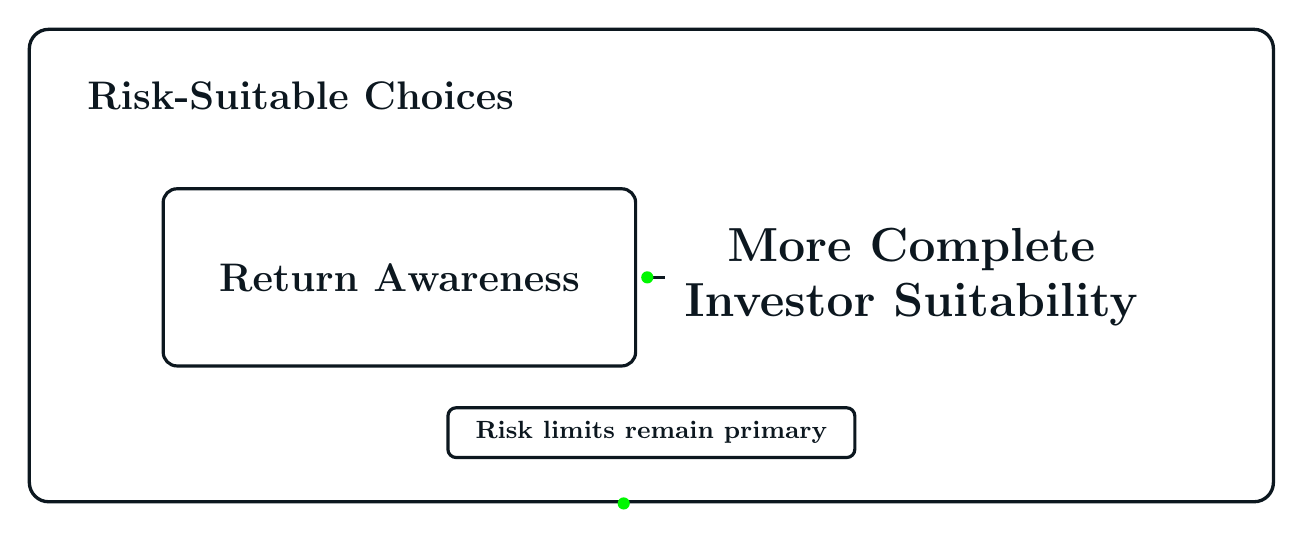
\begin{tikzpicture}
  \node[outer] (risk) {};
  \node[heading, anchor=north west] at ([xshift=18pt,yshift=-16pt]risk.north west)
    {Risk-Suitable Choices};

  \node[inner] (returns) at ([xshift=-3.2cm,yshift=-0.15cm]risk.center)
    {Return Awareness};

  \node[outcome] (outcome) at ([xshift=3.3cm,yshift=-0.15cm]risk.center)
    {More Complete\\Investor Suitability};

  \draw[navy, line width=1.15pt]
    ([xshift=0.35cm]returns.east) -- ([xshift=-0.35cm]outcome.west);
  \fill[green] ($(outcome.west)+(-0.35cm,0)$) circle (2.2pt);

  \node[guardrail, anchor=south] at ([yshift=16pt]risk.south)
    {Risk limits remain primary};
  \fill[green] ([xshift=-10pt]risk.south) circle (2.2pt);
\end{tikzpicture}
\end{document}
